%!TEX root = ../thesis_phd.tex
%%%%%%%%%%%%%%%%%%%%%%%%%%%%%%%%%%%%%%%%%%%%%%%%%%%%%%%%%%%%%%%%%%%%%%%%%%%%%%%%
% conclusion.tex:
%%%%%%%%%%%%%%%%%%%%%%%%%%%%%%%%%%%%%%%%%%%%%%%%%%%%%%%%%%%%%%%%%%%%%%%%%%%%%%%%
\chapter{Conclusion}
\label{conclusion_chapter}
%%%%%%%%%%%%%%%%%%%%%%%%%%%%%%%%%%%%%%%%%%%%%%%%%%%%%%%%%%%%%%%%%%%%%%%%%%%%%%%%

Even though it employs just a fraction the designed \nova exposure,
the neutrino oscillation result
presented in Chapter \ref{results_chapter} is nonetheless compelling.
The fit shows a slight preference for \textit{non-maximal} mixing,
that is, $\sin^2(\thetatth)$ not equal to 0.5.
If the best-fit value holds, future \nova measurements should be able to
resolve maximal mixing from non-maximal mixing.
Predicted sensitivity contours for the exposure in the \nova design
(six years, 14 kt, 700 kW) \cite{tdr}
are shown in Figure \ref{predicted_6yr_sensitivity}.

\begin{figure}
\begin{center}
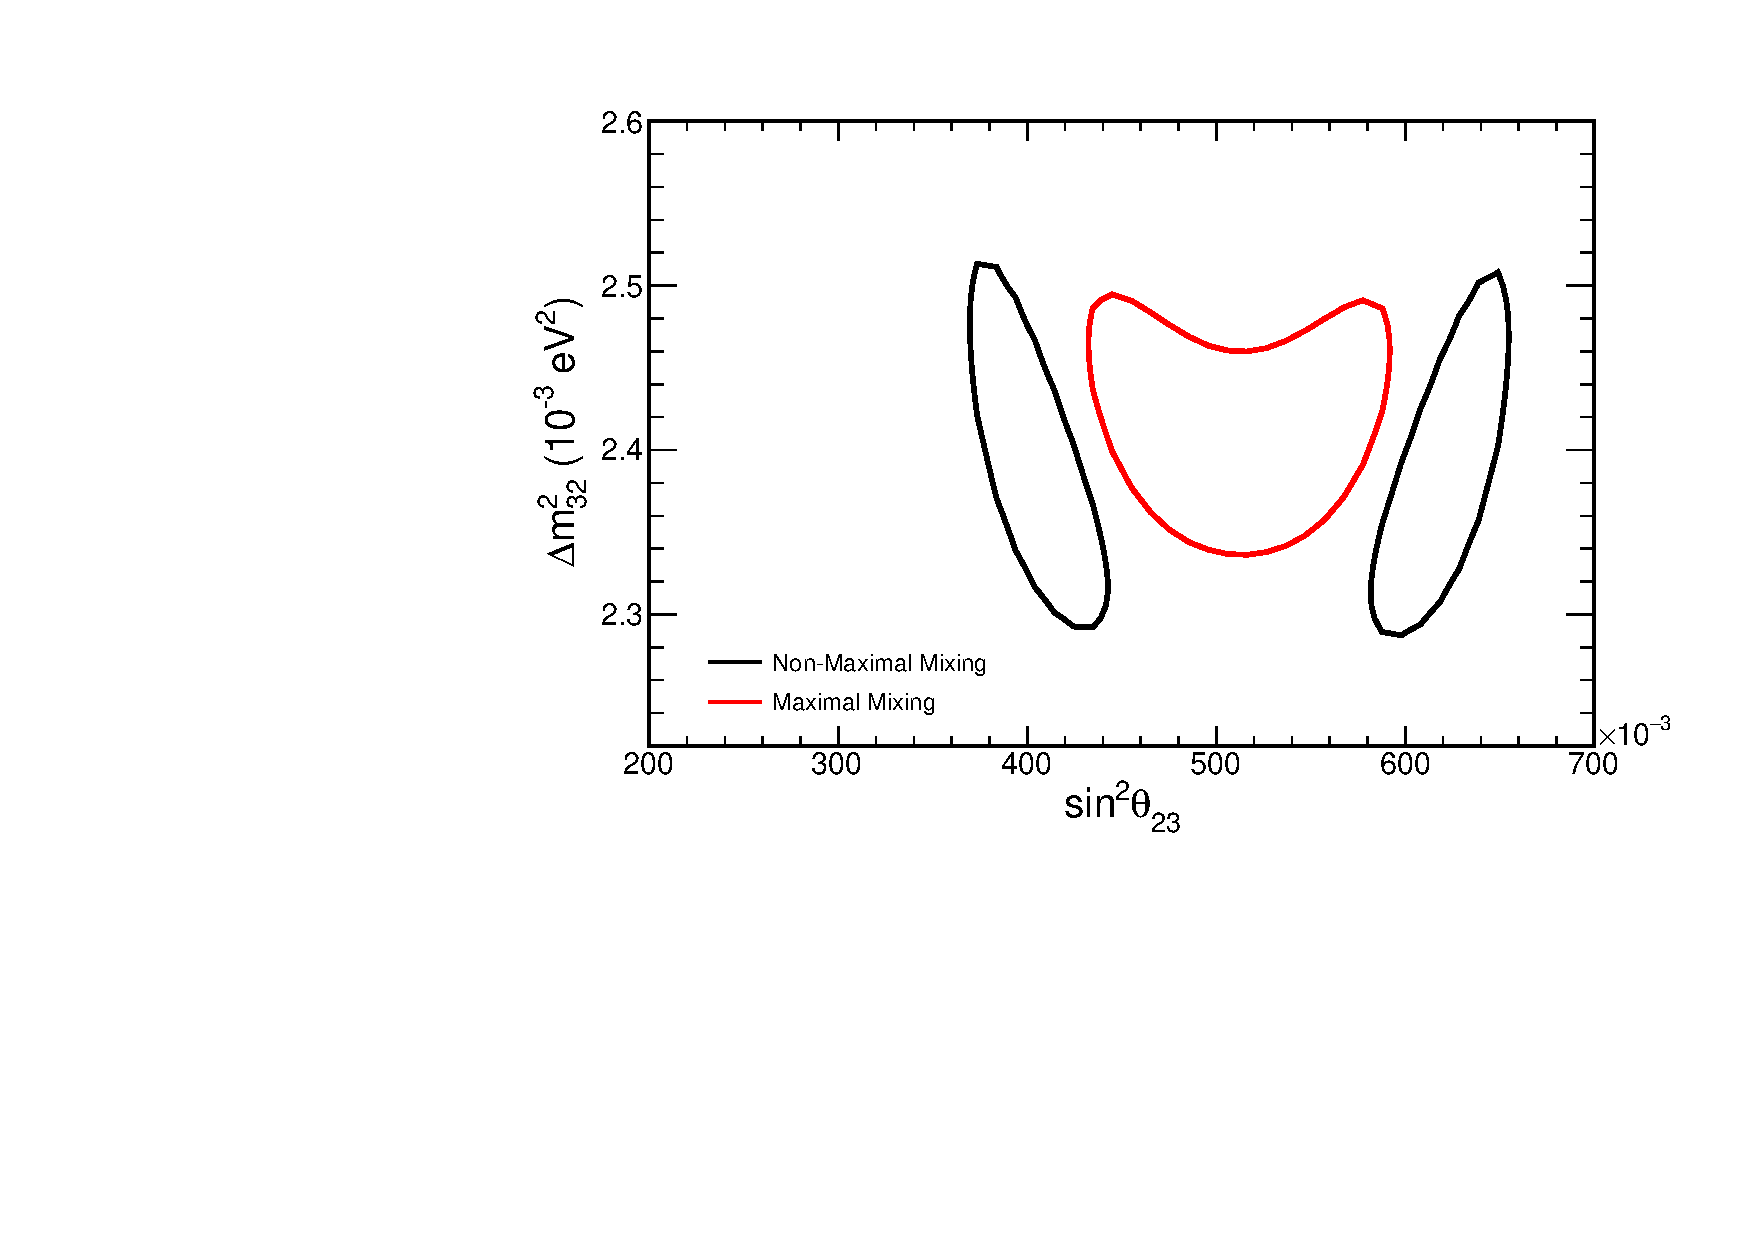
\includegraphics[width=\textwidth]{figures/results/contours6yr.pdf}
\end{center}
\caption{Predicted sensitivity of this analysis assuming \nova design exposure}{
\nova has been designed to run for six years with 14 kt of detector
mass and 700 kW operation of the \numi beam.
Assuming that exposure, the prediction above shows an ability
to resolve maximal mixing ($\sin^2(\thetatth)$ = 0.5), from a particular non-maximal mixing ($\sin^2(\thetatth)$ = 0.4) scenario.
}
\label{predicted_6yr_sensitivity}

\end{figure}



The selection technique presented here demonstrates a novel approach
to event classification.
While convolutional neural networks have delivered considerable
improvements to the field of computer vision and recognition
\cite{lecun2015deep},
the application to high-energy physics is completely new.
As shown in Chapter \ref{event_selection_chapter},
this technique offers improved physics sensitivity
through enhanced signal efficiency and background rejection
relative to traditional feature-extraction based approaches.

While the result shown here is compelling, additional effort could provide
further improvement.
The network architecture and training described in Chapter \ref{cnn_chapter}
has only been coarsely optimized.
Reconfiguration of the network -- for instance, removal of the aggressive
pooling in the early layers -- could improve the recognition
capability of the network.
It is also not clear that the learning capacity of the network has
been saturated; simply training the network through more iterations
could improve its performance.
Further, the event selection presented in
Chapter \ref{event_selection_chapter}
has also been only crudely optimized.
A grid-search optimization of the selection criteria based
on physics sensitivity could surely narrow the confidence intervals.
Perhaps better yet, a multivariate technique based on the background rejection
variables shown in Chapter \ref{background_rejection_section}
could be trained to take advantage of
correlations between those variables.

It should also be noted that the existing network can also
be used to improve the \nova \nue appearance measurement.
Studies have shown that this approach also promises improved
physics sensitivity for the measurement of $\delta$
and potential determination of the
neutrino mass hierarchy \cite{radovic2015cvn}.
It may also be possible to train convolutional neural networks
to solve other problems, for instance, identification
of reconstructed tracks and prongs.
The technique of semantic segmentation \cite{long2015fully},
where each pixel is given a classification label, could be especially
useful for that task.
Location of particular features in an event, such as an interaction
vertex, could also be achieved with a convolutional neural network.
Such an application would be analogous to facial-keypoint detection
\cite{lecun2015deep}.

The work presented here is clearly just the beginning.
\nova, with its fine-grained structure, provides a very interesting
testing ground for many techniques which are successful in
the field of computer vision.
From a physics perspective, the experiment
is also poised to deliver many compelling measurements in the coming
years.
The result shown here demonstrates a
vast potential for exciting developments on the road ahead.





%%%%%%%%%%%%%%%%%%%%%%%%%%%%%%%%%%%%%%%%%%%%%%%%%%%%%%%%%%%%%%%%%%%%%%%%%%%%%%%%
